\chapter{Zadanie 6}
Dalej zaprojektowany został automat stanów dla obiektu. Jego zadanie było proste ---
co określony okres czasu zmieniał wartości zadane obiektu. Jego implementacja
polegała na dodaniu zmiennej, w której trzymany był licznik, zwiększany z
każdym wywołaniem programu. Jeżeli licznik zawierał się w zadanym przedziale
wartości ustawiane były wartości zadane przypisane temu przedziałowi. Gdy
licznik wyszedł poza przewidziane przedziały, był zerowany. Przy okazji
w każdym z przedziałów ustawiana była inna zmienna, w której zapisany
był numer aktualnego stanu. Służyło to jedynie do wyświetlania na panelu
operatorskim aktualnego stanu. Czas przewidziany na jeden stan był łatwy do
wyznaczenia. Mając świadomość, iż program wywoływany jest raz na 4 sekundy,
długość przedziału pomnożona razy cztery była długością przebywania w danym
stanie w sekundach. Kod tego programu jest zawarty w listingu \ref{lst:automat}.
Panel operatorski, przedstawiający automat stanów przedstawia rysunek \ref{pic:automat}.

\begin{lstlisting}[style=customlatex,frame=single, caption=Kod automatu stanów, label=lst:automat]
cntr := cntr+ 1;
IF (cntr < 60) THEN
	stan := 1;
	Zadana_DMC2 := 36;
	Zadana_DMC3 := 37;
ELSIF (cntr< 120) THEN
	stan := 2;
	Zadana_DMC2 := 39;
	Zadana_DMC3 := 41;
ELSIF (cntr< 180) THEN
	stan := 3;
	Zadana_DMC2 := 35;
	Zadana_DMC3 := 34;
ELSIF (cntr< 240) THEN
	stan := 4;
	Zadana_DMC2 := 39;
	Zadana_DMC3 := 37;
ELSE
	cntr := 0;
END_IF;
\end{lstlisting}

\begin{figure}[tb]
  \centering
  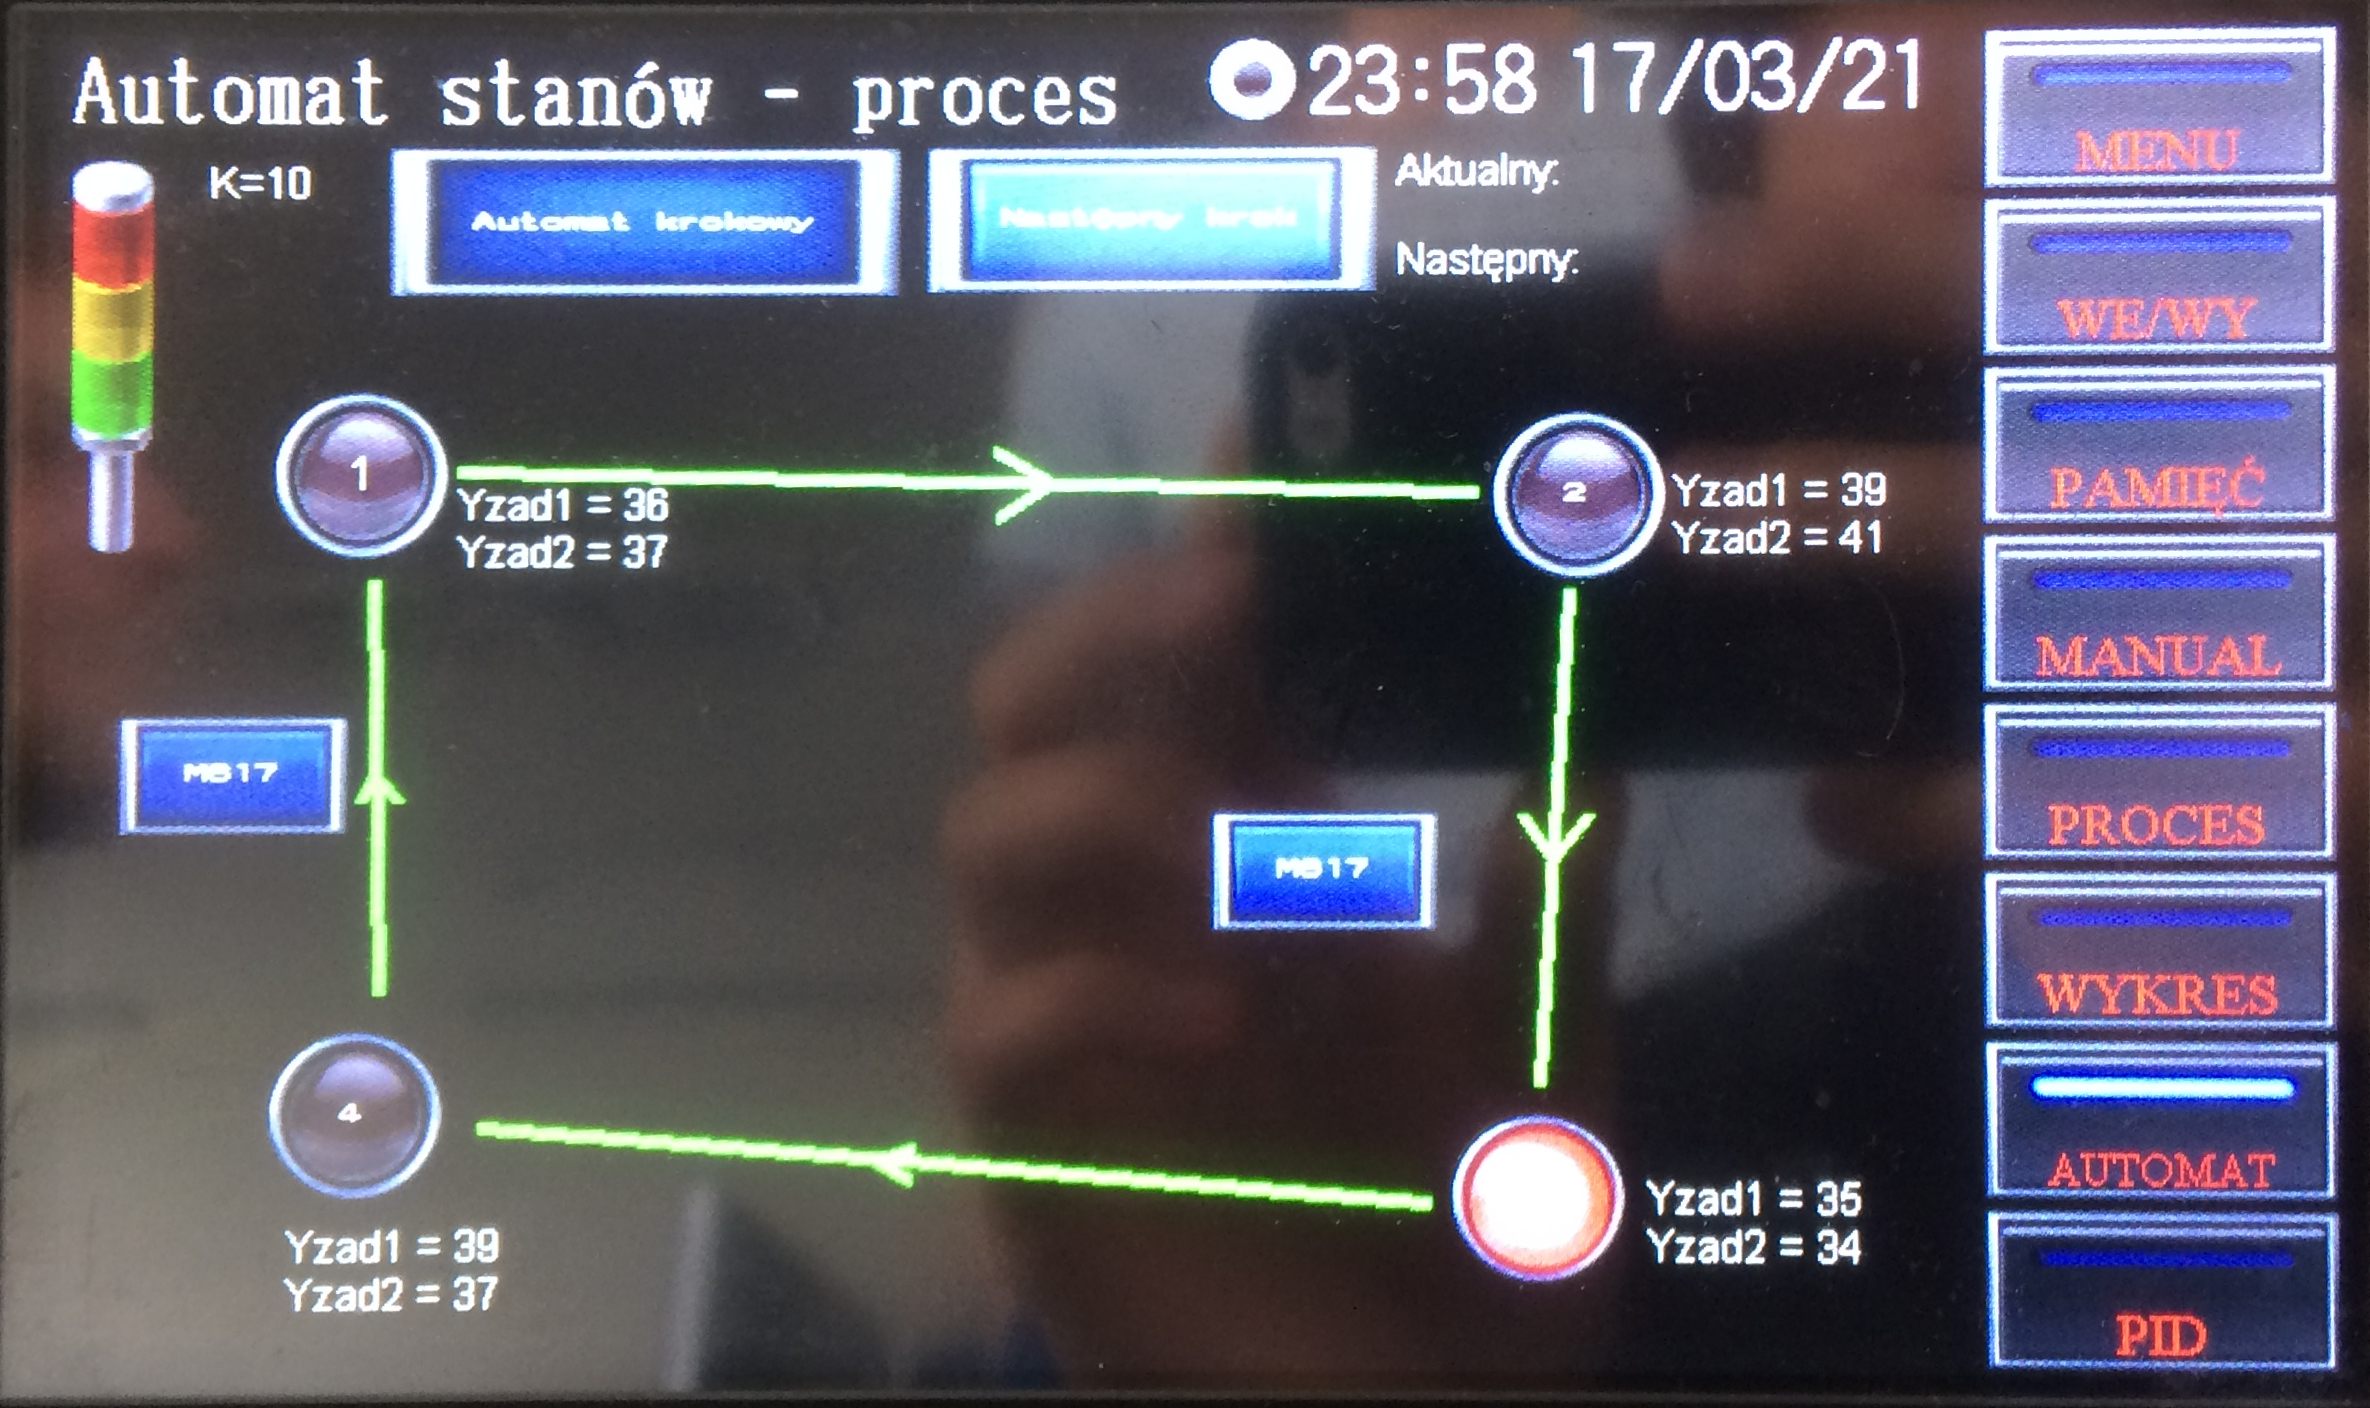
\includegraphics[width=0.9\textwidth]{Pictures/automat.jpg}
  \caption{Automat stanów}
  \label{pic:automat}
\end{figure}
